%%%%%%%%%%%%%%%%%%%%%%%%%%%%%%%%%%%%%%%%%%%%%%%%%%%%%%%%%%
%% Flujo de despliegue

\section{Integración y Distribución continua (CD/CI)}\label{pipeline:entrega-continua}

\subsection{Acerca del Pipeline o Flujo de entrega}\label{pipeline:acerca-del-pipeline}

Entendemos como pipeline (tubería) el conjunto de herramientas y procedimientos necesarios para transformar un commit de código a un output ejecutable que cumpla todos nuestros criterios de publicación. Es una cadena de producción automatizada ---como la de una fábrica--- que determina si el software se encuentra o no preparado para un lanzamiento, ajusta y empaqueta todas las dependencias necesarias del proyecto y genera los binarios para su distribución a los usuarios.

En esta cadena se ejecutarán de forma automática test unitarios, de integración, de rendimiento y todos los necesarios para determinar el estado actual del código en el repositorio. Por ejemplo, para comprobar mínimos de rendimiento se podría incorporar a nuestra pipeline un test de estrés para validar \lsc{FPS} mínimos.

Además de las pruebas, el sistema integrará todas las dependencias necesarias y empaquetará los binarios y cualquier recurso necesario para la distribución del programa a los sistemas de los clientes (win64, linux, android).

A nivel de gestión la pipeline nos permite determinar desde el primer momento los criterios de lanzamiento y organizar todo el flujo de trabajo en esa dirección evitando sorpresas y problemas de integración innecesarios. El tener un set herramientas y procedimientos para asegurar lanzamientos estables y funcionales desde el principio del proyecto es un activo fundamental para Bakumapu.

\subsubsection{Eficiencia}\label{pipeline:eficiencia}

Un factor muy importante con respecto al pipeline es la eficiencia total del proceso. Ya que queremos ser capaces de ejecutarlo múltiples veces al día se hace necesario \emph{optimizar el sistema para que no tarde más de 1 hora} de principio a fin (de commit a deploy). Este criterio de 1 hora otorgará márgen suficiente para que se pueda corregir o revertir cualquier commit que genere problemas; o al menos nos dará la información necesaria para su revisión o estudio.

\subsubsection{Repositorio de artefactos}

Entendemos como artefactos todos los binarios, librerías, resources y archivos necesarios para ejecutar correctamente el programa en un sistema operativo específico.

Dado que el uso de \lsc{GIT} para el control de binarios grandes trae complicaciones innecesarias se utilizará temporalmente una carpeta compartida de Google Drive mientras no sea necesario implementar una solución más robusta.

La carpeta compartida estará alojada en la siguiente dirección: \href{https://drive.google.com/drive/folders/15OtN9fs-UASOKTRcWGbR-knWMSmQGyO_?usp=sharing}. Será aquí donde se realizarán todos los deploy finales.

\subsection{Etapas de la pipeline}

Todo el proceso de la pipeline incluidos los test y compilación no debería tomar más de 5 minutos. Pasado ese tiempo el sistema debería arrojar error y se deben tomar medidas apropiadas para aumentar la eficiencia de sus procesos.

La pipeline contará con las siguientes etapas:

\begin{enumerate}
    \item Detectar nuevos commit en la rama \textbf{deploy}
    \item Comienza la compilación para las distintas plataformas.
    \item Deploy al repositorio de artefactos.
    \item Iniciar batería de test (unitarios, integración, análisis estático y rendimiento).
    \item En caso de error detener inmediatamente el sistema y generar log.
    \item El sistema permite merges de \textbf{deploy} a \textbf{release} solo si todos los test han sido superados exitosamente.
    \item Al detectar merges a \textbf{release} automáticamente subir los artefactos a los servidores públicos correspondientes (Steam, Play Store, etc.) para su distribución a clientes.
\end{enumerate}

\begin{figure}[ht]
	\centering
	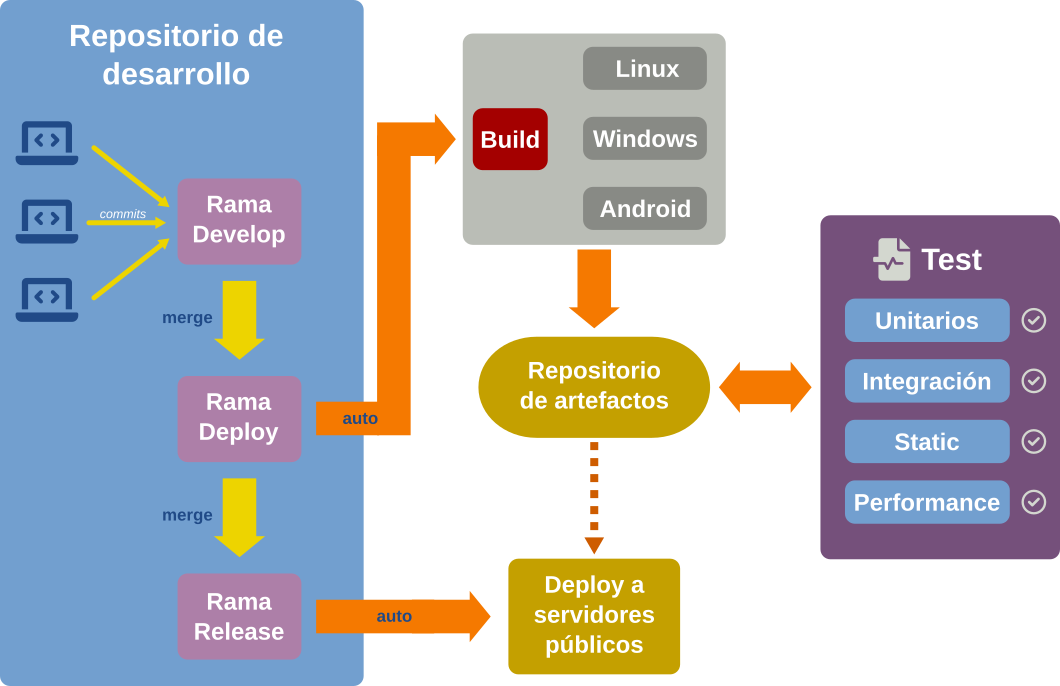
\includegraphics[width=\textwidth]{images/pipeline.png}
	\caption{Deploy Pipeline.}
\end{figure}

\subsection{Jenkins}

Para coordinar los scripts de automatización se utilizará Jenkins.

% =============================================================================

\subsection{Tipos de Test}\label{pipeline:tipos-de-test}

\begin{itemize}
  \item \textbf{Unit Test:} Test sencillos y específicos hechos para probar funciones o partes puntuales del código. Deberían correr en memoria y no llamar entidades externas como bases de datos, sistema de archivos, acceder a redes, etc. Lo importante es probar la unidad de código y no sus dependencias.
  \item \textbf{Integration Test:} Test que combinan secciones unitarias de código para comprobar que la interacción de sus distintos métodos funcionan correctamente.
  \item \textbf{Acceptance Test:} Se prueba el software y el sistema al completo desde el punto de vista de un agente externo al desarrollo revisando que el programa satisfaga todas las especificaciones del usuario.
  \item \textbf{Performance Test:} Se revisa que el software cumpla tiempos de respuesta, estabilidad y \lsc{FPS}.
  \item \textbf{Static Analysis:} 
  \item \textbf{Sign-Offs: Regulaciones:} 
  \item \textbf{Security Test:} 
  \item \textbf{Scalability Test:} 
\end{itemize}

Exportar a Linux, Windows y Android:

Linux:
\begin{lstlisting}
$ godot --no-window --export-debug "Linux" export/linux/Bakumapu.x86_64
\end{lstlisting}

Windows:
\begin{lstlisting}
$ godot --no-window --export-debug "Windows" export/windows/Bakumapu.exe
\end{lstlisting}

Android:
\begin{lstlisting}
$ godot --no-window --export-debug "Android" export/android/Bakumapu.apk
\end{lstlisting}
